\begin{frame}
    \frametitle{Introduction}
    \framesubtitle{Problems with Diffusion Models}
    
    \begin{columns}
        \column{0.5\textwidth}
        \centering
        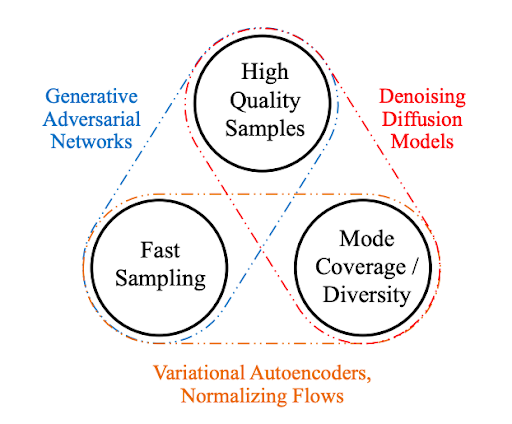
\includegraphics[width=0.9\textwidth]{images/GANs_Diffusion_Autoencoders.png}
    
        \column{0.5\textwidth}
        \centering
        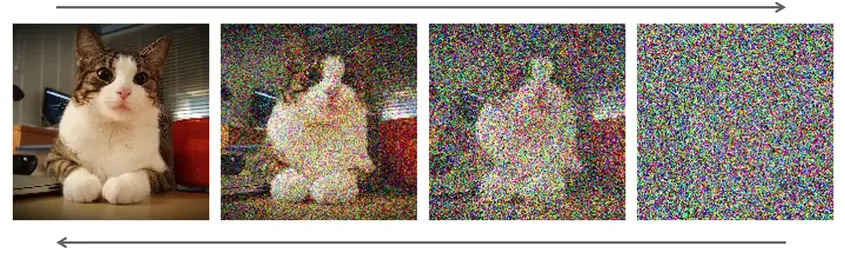
\includegraphics[width=\textwidth]{images/Generation-with-Diffusion-Models-ezgif.com-webp-to-jpg-converter.jpg}
      \end{columns}  
      \tiny{\footnotemark \url{https://developer.nvidia.com/blog/improving-diffusion-models-as-an-alternative-to-gans-part-1/}}
      \tiny{\footnotemark \url{https://miro.medium.com/v2/resize:fit:720/format:webp/1*RDPhd2dvmHE4UrAP-QHb9w.png}}
    \end{frame}
    
    % ---------- Proposed solutions ----------
    \begin{frame}
    \frametitle{Introduction}
    \framesubtitle{Proposed solutions}
    \begin{itemize}
        \item One-step image-to-image translation method for paired and unpaired settings
        \item Reduce number of inference steps to 1
        \item Trainable without image pairs
        \item Adapt pre-trained text-conditional one-step diffusion model to new domains via adversarial learning
    \end{itemize}
\end{frame}